\subsection{Coulomb differential cross sections}
The Coulomb differential cross section describes the collisions that charged particles experience in a medium as a result of interactions with the charges of the background charged particles present in the plasma. The unscreened and screened Coulomb differential cross sections are found by solving the Schr\"{o}dinger equation, that is solutions to,
\begin{equation} \label{eqn:Schrodinger}
    \left[-\dfrac{\hbar^2}{2 m}\nabla^2 + k^2 + V(r)\right] \Psi_k(\vec{r}) = \dfrac{(\hbar \vec{k})^2}{2m} \Psi_k(\vec{r}),
\end{equation}
where $m$ is the reduced mass, $k$ is the wave number of the incident particle, and $V(r)$ is the interaction potential. Solutions to Eq. \eqref{eqn:Schrodinger} have at large distances from center of the potential the asymptotic form 
\begin{equation}  \label{eqn:asymptotic-solution}
    \Psi \approx \text{e}^{i\,k\,z} + \dfrac{f(\theta)}{r}\text{e}^{i\,k\,r}
\end{equation}
where the first term describes the incident particle traveling in the positive direction of the z-axis. The second term in Eq. \eqref{eqn:asymptotic-solution} describes the scattered particles as a spherical wave emitted where $f(\theta)$ is some function of the scattering angle characteristic of the interaction potential. In Eq. \eqref{eqn:asymptotic-solution}, $f(\theta)$ is often referred to as the scattering amplitude. The differential cross section corresponding to the solution to Eq. \eqref{eqn:Schrodinger} is then found by taking the ratio of the probability per unit time that the scattered particle pass through a surface element $dS = r^2 d\Omega$ to the current density of the incident wave, that is,
\begin{equation} \label{eqn:formula-distinguishable-particles}
    \sigma(E,\theta) = |f(\theta)|^2.
\end{equation}

Collisions where two identical particles collide requires special consideration. This is due to the identity of the particles making it impossible to say which of the particle is scattered and which is recoiling. The differential cross section that describes the interaction of identical particles is
\begin{equation} \label{eqn:formula-identical-particles}
    \sigma_{i}^{C} = | f(\theta) |^2 + | f(\pi - \theta) |^2 + \dfrac{(-1)^{2s}}{2s+1} \left[ f(\theta) f^{\star}(\pi-\theta) + f^{\star}(\theta) f(\pi-\theta) \right],
\end{equation}
where $s$ is the spin of the particles. The first term in Eq. \eqref{eqn:formula-identical-particles} describes the forward scattering probability,while the second term describes the backward scattering probability. The third term in Eq. \eqref{eqn:formula-identical-particles} is an interference term and characterizes the exchange interaction between the forward and backward directions.

The un-screened interaction potential for two charged particles is described by the standard Coulomb potential,
\begin{equation} \label{eqn:Coulomb_potential}
    V(r) = \dfrac{Z_1 \, Z_2 \, e^2}{r},
\end{equation}
where $Z_1 e$ and $Z_2 e$ are the charges of the incident and target charged particles, and $r$ is the distance between the two charges. Note that the Coulomb potential allows for particles that are infinitely far apart to interact with one another, due to the $1/r$ term in Eq. \eqref{eqn:Coulomb_potential}. Solving Schr\"{o}dinger's equation with the Coulomb potential yields the following scattering amplitude in Coulomb units,
\begin{equation} \label{eqn:coulomb-scattering-amplitude}
    f(\theta) = \dfrac{\gamma}{2 \, k \, \sin^2 \theta/2} \exp \left[ 2 \, i \, \gamma \, \log \sin \theta/2 \right] \dfrac{\Gamma(1 + i/k)}{\Gamma(1 - i/k)},
\end{equation}
where $\gamma = Z_1 \, Z_2 \, e^2 / \hbar \, v$, $v$ is the incident velocity, $\hbar \, k = m_r \, v$, and $m_r = \frac{m_1 m_2}{m_1 + m_2}$ is the reduced mass of the system. Substituting Eq. \eqref{eqn:coulomb-scattering-amplitude} into Eqs. \eqref{eqn:formula-distinguishable-particles} and Eq. \eqref{eqn:formula-identical-particles} yields the differential cross sections corresponding to an unscreened Coulomb potential for distinguishable and identical particle scattering collisions. In the following, both the distinguishable and identical unscreened Coulomb differential cross sections are examined.

The unscreened Coulomb differential cross section is found by substituting Eq. \eqref{eqn:coulomb-scattering-amplitude} into Eq. \eqref{eqn:formula-distinguishable-particles},
\begin{equation} \label{eqn:dist_unscreened_coulomb}
    \sigma_{d}^{C} = \left(\dfrac{Z_1 \, Z_2 \, e^2}{2 \, m_r \, v^2}\right)^2 \dfrac{1}{\sin^4 \theta/2},
\end{equation}
Eq. \eqref{eqn:dist_unscreened_coulomb} can is written in a more usable form by rewriting $e^2 = \alpha \, \hbar c$ and using the half angle trigonometry identity $2 \sin^2 \theta / 2 = 1 - \cos \theta$ to give
\begin{equation} \label{eqn:coulomb-dcs}
    \sigma_{d}^{C}(E,\mucm) = \left(\dfrac{Z_1^2 \, Z_2^2 \, \left(\alpha \, \hbar c\right)^2}{ 4 \, E^2 \, \left(\frac{A}{1 + A} \right)^2}\right) \dfrac{1}{(1 - \mucm)^2}, \quad A = \dfrac{m_2}{m_1}
\end{equation}

Figure \ref{fig:sigma_c} shows a plot of Eq. \eqref{eqn:coulomb-dcs} for deuterons colliding with tritons at an incident energy of $1 \mev$ cutoff at $\mucm = 0.99$. Looking at Figure \ref{fig:sigma_c} the Coulomb differential cross section for distinguishable particles is highly peaked about $\mucm = 1$, meaning that particles will most likely undergo collisions that result in zero angular deflection/energy loss. This peakedness is due to the fact that Eq. \eqref{eqn:coulomb-dcs} has a singularity as $\mucm \rightarrow 1$ as a result of the Coulomb interaction potential which allows particles that are infinitely far apart to nonphysically interact with one another. As a result of the singularity Eq. \eqref{eqn:coulomb-dcs} cannot be integrated over the entire range of $\mucm$, and instead must be cutoff at some cosine angle close to one. 
\begin{figure}[!htb]
    \centering
    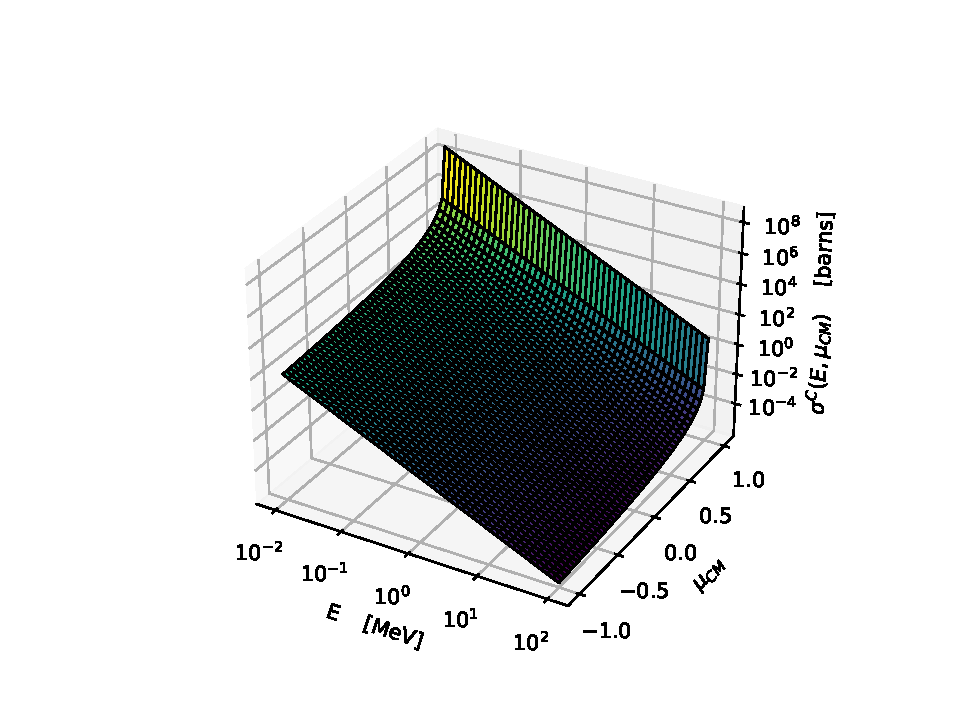
\includegraphics[scale=1.00]{../figures/chapter-4/sigma-C.pdf}
    \caption{Distinguishable Coulomb differential cross section for energetic deuterons colliding with background tritons cutoff at $\mucm = 0.99$}
    \label{fig:sigma_c}
\end{figure}

The total scattering cross section associated with Eq. \eqref{eqn:coulomb-dcs} is found by integrating over $\mucm$ from $-1$ to some cutoff angle, $\mu_{cut}$ resulting in the following total scattering cross section
\begin{equation} \label{eqn:unscreened-total-xs}
    \sigma^C_d(E) = \left(\dfrac{Z_1^2 \, Z_2^2 \, \left(\alpha \, \hbar c\right)^2}{ 4 \, E^2 \, \left(\frac{A}{1 + A} \right)^2}\right) \dfrac{\mu_{cut}}{1-\mu_{cut}}, \quad \text{where} \,\, -1 < \mu_{cut} < 1.
\end{equation}
Figure \ref{fig:sigma_c_total} shows Eq. \eqref{eqn:unscreened-total-xs} for several different collisions and with a cutoff cosine of $\mu_{cut} = 0.999$. From Figure \ref{fig:sigma_c_total} as the energy of the incident particle increases the magnitude of the total cross section decreases, this can also be seen in Figure \ref{fig:sigma_c}. Additionally, as the mass of the incident particle increases so does the magnitude of the total cross section. Conversely, as the mass of the target particle increases, the magnitude of the of the total cross section decreases. Lastly, for nominal ICF energies, $<10$ MeV, the magnitude of Eq. \eqref{eqn:unscreened-total-xs} is large meaning that for typical ICF densities the mean free path is very small and highly peaked about zero angular deflection.
\begin{figure}[!htb]
    \centering
    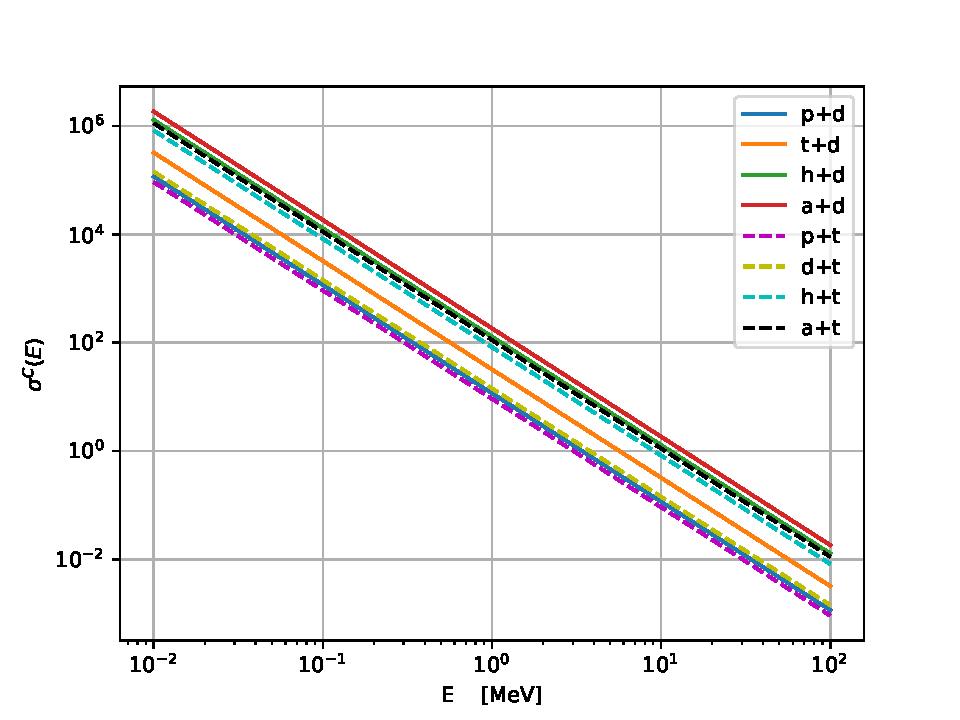
\includegraphics[scale=0.75]{../figures/chapter-4/total-sigma-C.pdf}
    \caption{Total distinguishable Coulomb differential cross section for several collisions cutoff at $\mucm = 0.999$}
    \label{fig:sigma_c_total}
\end{figure}

The identical particle unscreened Coulomb differential cross section is found by substituting Eq. \eqref{eqn:coulomb-scattering-amplitude} into Eq. \eqref{eqn:formula-identical-particles} giving,
\begin{multline} \label{eqn:coulomb-unscreened-identical}
   \sigma_{i}^{C} = \dfrac{\gamma^2}{k^2} \left[ \dfrac{1}{(1 - \mucm)^2} + \dfrac{1}{(1 + \mucm)^2} \right. \\ \left. + \dfrac{(-1)^{2s}}{2s+1} \dfrac{2}{(1 - \mucm)(1 + \mucm)} \cos \left( \gamma \, \log \, \dfrac{1 - \mucm}{1 + \mucm} \right) \right].
\end{multline}
Figure \ref{fig:coulomb-identical} shows $\sigma_{C,i}$ for a variety of incident particle energies and cosine of CM scattering angles. In Figure \ref{fig:coulomb-identical} it is clear that the identical particle Coulomb differential cross section is highly peaked about $\mucm = -1, 1$. When comparing the distinguishable and identical differential cross sections we see that both differential cross section are highly peaked about $\mucm = 1$ meaning that it is highly likely that the initial particle will scatter in the forward direction in both identical and distinguishable collisions; however, the identical particle differential cross section is highly peaked about $\mucm = -1$ meaning that it is very likely that the incident particle will transfer all of it's energy to the target particle. This means that the recoil now looks exactly like the incident particle underwent a small angle deflection collision.
\begin{figure}[!htb]
    \centering
    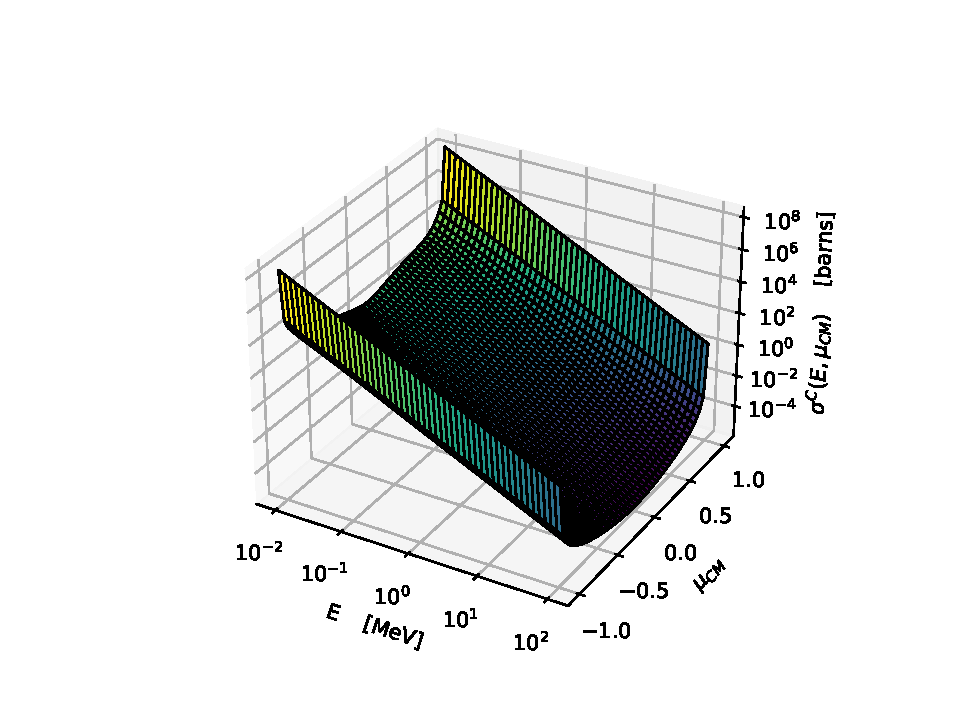
\includegraphics[scale=1.00]{../figures/chapter-4/sigma-Ci.pdf}
    \caption{The identical particle Coulomb differential cross section for deuterons colliding with background deuterons for $\mucm = [-0.99,0.99]$}
    \label{fig:coulomb-identical}
\end{figure}

Eq. \eqref{eqn:coulomb-unscreened-identical} can be greatly simplified when $\gamma \ll 1$ meaning that the velocity of the incident particle is so large that $\hbar v \gg Z_1 Z_2 e^2$. In this case the cosine in the third term can be replaced by unity and Eq. \eqref{eqn:coulomb-unscreened-identical} becomes
\begin{equation} \label{eqn:coulomb-unscreened-identical-simplified}
   \sigma_{i}^{C} \approx \dfrac{2 \, \gamma^2}{k^2 (1 - \mucm^2)} \left[\dfrac{1+ \mucm^2}{1-\mucm^2} + \dfrac{(-1)^{2s}}{2s+1}\right], \quad \text{when} \,\, \gamma \ll 1.
\end{equation}
For the opposite case, $\hbar v \ll Z_1 Z_2 e^2$, the cosine term in Eq. \eqref{eqn:coulomb-unscreened-identical} is a rapidly oscillating function, and the resulting cross section differs significantly from the Rutherford value given by Eq. \eqref{eqn:coulomb-unscreened-identical-simplified}. Figure \ref{fig:coulomb-identical-2d} shows the oscillations in the differential cross section due to the cosine term at various incident particle energies. In Figure \ref{fig:coulomb-identical-2d} it is clear that at low energies ($E < 10$ keV) these oscillations are significant; however, at higher energies these oscillations atr not significant and the Eq. \eqref{eqn:coulomb-unscreened-identical} rapidly approaches Eq. \eqref{eqn:coulomb-unscreened-identical-simplified}.

\begin{figure}[!htb]
    \centering
    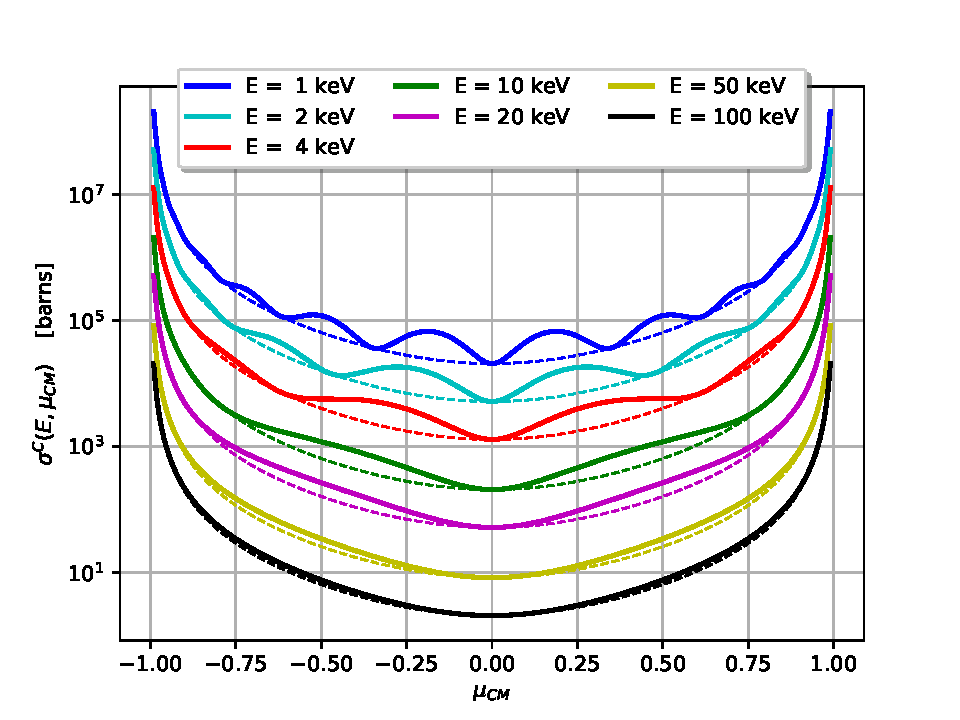
\includegraphics[scale=0.75]{../figures/chapter-4/sigma-Ci-2d.pdf}
    \caption{Comparison between the full (solid lines) and approximate (dashed lines) identical particle Coulomb differential cross sections at various energies for tritons colliding with background tritons for $\mucm = [-0.99,0.99]$.}
    \label{fig:coulomb-identical-2d}
\end{figure}

% ------------------------------------------------
% SCREENING FUNCTIONS 
% ------------------------------------------------
\subsubsection{The Yukawa potential}
Here the Yukawa potential is introduced as a reasonable form of screening in plasmas. To introduce the concept of Debye shielding consider a finite temperature plasma consisting of a statistically large number of electrons and ions and by assuming that the ion and electron densities are initially equal and spatially uniform. The ions and electrons in the background plasma have random thermal motion, thermally induced pertubations about the equilibrium will cause small, transient spatial variations of the electrostatic potential $\phi$. Next, the following assumptions are made:
\begin{enumerate}
    \item The background plasma is assumed to be nearly collisionless so that collisions between particles may be neglected
    \item Each species, denoted as $i$, may be considered as a ``fluid'' having a density $n_i$, and a temperature $T_i$, a pressure $P_i = n_i \kappa T_i$, and a mean a velocity $\boldsymbol{u}_i$ so that the collisionless equation of motion for each fluid is
    \begin{equation} \label{eqn:collisionless-motion}
        m_i \dfrac{d \boldsymbol{u}_i}{dt} = q_i \boldsymbol{E} - \dfrac{1}{n_i} \nabla P_i
    \end{equation}
    where $m_i$ is the particle mass, $q_i$ is the charge of a particle, and $\boldsymbol{E}$ is the electric field.
\end{enumerate}

Now consider a perturbation with a sufficiently \textit{slow} time dependence to allow the following assumptions:
\begin{enumerate}
    \item The inertial term $\approx d/dt$ on the left-hand side Eq. \eqref{eqn:collisionless-motion} is negligible and may be dropped.
    \item Inductive electric fields are negligible so the electric field is almost entirely electrostatic, i.e., $\boldsymbol{E} \approx - \nabla \phi$.
    \item All temperature gradients are smeared out by thermal particle motion so that the temperature of each species is spatially uniform
    \item The plasma remains in thermal equilibrium throughout the perturbation
\end{enumerate}
Invoking these approximations, Eq. \eqref{eqn:collisionless-motion} reduces to
\begin{equation} \label{eqn:pressure-balance}
    0 \approx -n_i q_i \nabla \phi - \kappa T_i \nabla n_i,
\end{equation}
which is a simple balance equation between the force due to the electrostatic electric field and the force due to the isothermal pressure gradient. Eq. \eqref{eqn:pressure-balance} is readily solved to give the Boltzmann relation
\begin{equation} \label{eqn:boltzmann-relation}
    n_i = n_{i,0} \exp\left(-q_i \phi / \kappa T_i\right),
\end{equation}
where $n_{i,0}$ is a constant. It is important to note that Eq. \eqref{eqn:boltzmann-relation} results from the assumption that the perturbation is \textit{very slow}; if this is not the case, then inertial effects, inductive electric fields, or temperature gradient effects will cause the plasma to have completely different behavior than the Boltzmann relation.

Next, imagine \textit{slowly} inserting a single additional particle with charge $q_T$ into an initially unperturbed, spatially uniform, neutral plasma. To keep the algebra simple, the origin of the coordinate system is defined to be at the location of the test particle. Before insertion of the test particle, the plasma potential was $\phi = 0$ everywhere because the ion and electron densities were spatially uniform and equal, but now the ions and electrons will be perturbed because of their interaction with the test particle. Particles having the same polarity as $q_T$ will be slightly repelled whereas particles of opposite polarity will be slightly attracted. This slight displacement resulting from these repulsions and attractions will result in a small, but finite, potential in the plasma.

This slight displacement of plasma particles is called \textit{shielding} or \textit{screening} of the test particle because the displacement tends to reduce the effectiveness of the test particle field. As an example, suppose the test particle is a positively charged ion which when inserted into the plasma attracts the nearby electrons and repels the ions. The net result is a negative charge cloud surrounding the test particle which effectively shields the test particles potential from the rest of the plasma.

The screening effect is calculated using Poisson's equation with the source terms being the test particle and its associated cloud. The cloud contribution is determined using the Boltzmann relation for the particles that participate in the screening. This is a ``self-consistent'' calculation for the potential because the shielding cloud is affected by its self-potential.

Thus, Poisson's equation becomes
\begin{equation} \label{eqn:poisson-relation}
    \nabla^2 \phi = - \dfrac{1}{\epsilon_0} \left[q_T \delta(\boldsymbol{r}) + \sum\limits_{i} n_i(\boldsymbol{r}) q_i\right],
\end{equation}
where the term $q_T \delta(\boldsymbol{r})$ on the right-hand side represents the charge density due to the test particle and the term $\sum\limits_{i} n_i(\boldsymbol{r}) q_i$ represents the charge density of all plasma particles that participate in the screening. Because the test particle was inserted slowly, the plasma response will be Boltzmann-like and we may substitute Eq. \eqref{eqn:boltzmann-relation} into Eq. \eqref{eqn:poisson-relation}. Additionally, because the perturbation due to a single test particle is infinitesimal, it can be assumed that $|q_i \phi| \ll \kappa T_i$, reducing Eq. \eqref{eqn:poisson-relation} to 
\begin{equation} \label{eqn:poisson-relation-2}
    \nabla^2 \phi = - \dfrac{1}{\epsilon_0} \left[q_T \delta(\boldsymbol{r}) + \sum\limits_{i} n_{i,0} q_i \left(1 - \dfrac{q_i \phi}{\kappa T_i}\right) \right]
\end{equation}
The assumption of initial neutrality means that $n_{e0}q_e + \sum\limits_{i} n_{i,0} q_i = 0$, in which case Eq. \eqref{eqn:poisson-relation-2} reduces to
\begin{equation} \label{eqn:poisson-relation-3}
    \nabla^2 \phi - \dfrac{1}{\lambda_D^2} \phi = - \dfrac{q_T}{\epsilon_0} \delta(\boldsymbol{r})
\end{equation}
where the effective Debye length is defined by
\begin{equation}
    \dfrac{1}{\lambda_D^2} = \sum\limits_i \dfrac{1}{\lambda_i^2}
\end{equation}
and the species Debye length $\lambda_i$ is
\begin{equation}
    \lambda_i^2 = \dfrac{\epsilon_0 \kappa T_i}{n_{i0}q_i^2}.
\end{equation}
Finally Eq. \eqref{eqn:poisson-relation-3} can be solved to give
\begin{equation} \label{eqn:yukawa-potential}
    \phi(\boldsymbol{r}) = \dfrac{q_T}{4 \pi \epsilon_0 r} \text{e}^{-r/\lambda_D};
\end{equation}
this is sometimes called the Yukawa potential. In Eq. \eqref{eqn:yukawa-potential} the exponential term decreases more rapidly than the $1/r$ term thereby making the probability that particles will experience interactions at distances much greater than $R$ impossible. This leads to an interaction potential that is finite as $r \rightarrow \infty$ while still possessing the same general behavior as the original Coulomb interaction potential.

% ------------------------------------------------
% SCREENED COULOMB DIFFERENTIAL CROSS SECTIONS 
% ------------------------------------------------
\subsubsection{Screened coulomb differential cross sections}
Using the Yukawa potential derived in the previous section, the screened Coulomb differential cross section can be derived. The Schr\"{o}dinger equation with the Yukawa potential cannot be solved exactly and therefore its solution is approximated with the Born approximation. The Born approximation consists of approximating the the scattered wave function by a plane wave, and gives the following formula for the scattering amplitude
\begin{equation} \label{eqn:first-born-approximation}
    f(\theta) \approx - \dfrac{2 \, m}{\hbar^2} \int\limits_0^{\infty} U(r) \, \dfrac{\sin qr}{q} \, r \, dr
\end{equation}
where $q = 2 \, k \, \sin \theta / 2$. Substituting the screened interaction potential into Eq. \eqref{eqn:first-born-approximation} and yields
\begin{equation} \label{eqn:wentzel-scattering-amplitude}
    f_s(\theta) = \dfrac{Z_1 \, Z_2 \, e^2 \, m}{2 \, k^2 \, \hbar^2} \dfrac{1}{(2kR)^{-2} + \sin^2 \theta/2} = \dfrac{\gamma}{2 \, k} \left[\dfrac{1}{(2kR)^{-2} + \sin^2 \theta/2}\right].
\end{equation}
In Eq. \eqref{eqn:wentzel-scattering-amplitude} the term $(2kR)^{-2}$ is often referred to as the screening parameter and is denoted by $A_s$. Note that as $A_s \rightarrow 0$ Eq. \eqref{eqn:wentzel-scattering-amplitude} approaches the unscreened Coulomb potential scattering amplitude, Eq. \eqref{eqn:Coulomb_potential}, without the exponential and gamma function terms. In fact it has been shown that the Born approximation is not a valid approximation of the scattering amplitude when a screened interaction potential is used for nucleon-nucleon interactions unless the incident particles energy is at relativistic speeds. Nonetheless, the differential cross sections for distinguishable and identical particles are derived using Eq. \eqref{eqn:wentzel-scattering-amplitude} as they result in differential cross sections that are at least finite at $\mucm = 1$ and resemble the Coulomb differential cross sections previously derived.

Using Eqs. \eqref{eqn:formula-distinguishable-particles} and \eqref{eqn:formula-identical-particles} the screened Coulomb differential cross section for distinguishable and identical particles are
\begin{equation} \label{eqn:screened-coulomb-d}
    \sigma_{d}(E,\mucm) = \dfrac{\gamma^2}{k^2} \dfrac{1}{\left[A_s + 1 - \mucm\right]^2},
\end{equation}
and
\begin{multline} \label{eqn:screened-coulomb-i}
    \sigma_{i}(E,\mucm) = \dfrac{\gamma^2}{k^2} \left[ \dfrac{1}{\left(A_s + 1 - \mucm\right)^2} + \dfrac{1}{\left(A_s + 1 + \mucm\right)^2} \right. \\ \left. + \dfrac{(-1)^{2s}}{2s+1} \dfrac{2}{\left(A_s + 1 - \mucm\right)\left(A_s + 1 + \mucm\right) }\right].
\end{multline}
In Eq. \eqref{eqn:screened-coulomb-d} as $A_s \rightarrow 0$ it becomes the unscreened Coulomb differential cross sections (Eq. \eqref{eqn:coulomb-dcs}). However, in the identical particle case as $A_s \rightarrow 0$ instead of approaching the unscreened identical particle differential cross Eq. \eqref{eqn:screened-coulomb-i} becomes the approximate unscreened identical particle differential cross section (Eq. \eqref{eqn:coulomb-unscreened-identical-simplified}). This discrepancy is due to the validity of the Born approximation, which is only valid if the incident particle has high energy. However, Eqs. \eqref{eqn:screened-coulomb-d} and \eqref{eqn:screened-coulomb-i} are considered ``good enough'' approximations to the true differential cross section and are used throughout the remainder of this dissertation. 

